% TEMPLATE for Usenix papers, specifically to meet requirements of
%  USENIX '05
% originally a template for producing IEEE-format articles using LaTeX.
%   written by Matthew Ward, CS Department, Worcester Polytechnic Institute.
% adapted by David Beazley for his excellent SWIG paper in Proceedings,
%   Tcl 96
% turned into a smartass generic template by De Clarke, with thanks to
%   both the above pioneers
% use at your own risk.  Complaints to /dev/null.
% make it two column with no page numbering, default is 10 point

% Munged by Fred Douglis <douglis@research.att.com> 10/97 to separate
% the .sty file from the LaTeX source template, so that people can
% more easily include the .sty file into an existing document.  Also
% changed to more closely follow the style guidelines as represented
% by the Word sample file. 

% Note that since 2010, USENIX does not require endnotes. If you want
% foot of page notes, don't include the endnotes package in the 
% usepackage command, below.

% This version uses the latex2e styles, not the very ancient 2.09 stuff.
\documentclass[letterpaper,twocolumn,10pt]{article}
\usepackage{usenix,epsfig,url}
\begin{document}

%don't want date printed
\date{}

%make title bold and 14 pt font (Latex default is non-bold, 16 pt)
\title{\Large \bf Webcam Fuzz Testing: Testing IoT Deployments}

%for single author (just remove % characters)
\author{
{\rm Matthew Elbert}\\
University of Utah
\and
{\rm Jeffrey Kitchen}\\
University of Utah
% copy the following lines to add more authors
% \and
% {\rm Name}\\
%Name Institution
} % end author

\maketitle

% Use the following at camera-ready time to suppress page numbers.
% Comment it out when you first submit the paper for review.
\thispagestyle{empty}


\subsection*{Abstract}
Fuzz testing, or fuzzing, is a simple method to find bugs and vulnerabilities in programs. We use fuzzing methods to attempt to identify security vulnerabilities in two Wi-Fi cameras. 

\section{Introduction}
\subsection{Motivation}

Fuzz testing is a method of testing in which random, potentially invalid inputs are sent to a program or service in order to test for vulnerabilities. It is often used as either a gray or black-box testing platform for security testing. Fuzz testing can be a very cheap and effective implementation of testing as many inputs can be generated, sent, and analyzed automatically, without the need for a human to monitor. However, a truly random test input could easily not provide anything useful in a reasonable amount of time. Therefore, many solutions (citations needed) propose a different method where random mutation of good inputs is used so that requests that are close to being correct are used. 
Because the world has become more internet-connected than ever, fuzz testing can be an important tool for developers as network-facing interfaces can experience any input, and need to be tested for this randomness. However, many functions are very state-driven, and a true, random test may only test a single interface, and not the whole system. Because of this, many of these fuzz testers must be stateful in order to do a complete test. Because of many security issues with the current Internet architecture, there are obviously some security measures put in place to almost anything that is deployed on a network, even if it is meant to only be local. Therefore, something as simple as logging into an interface needs to be taken into account in order to get more meaningful tests.

\subsection{Problem}

In this project, we designed, implemented and evaluated an automated tester for a networking service. This is meant to evaluate the value of fuzz testing on a network, with the goal of hopefully finding a previously undiscovered bug. A very basic and highly proliferated technology deployed on the internet is an HTTP server. But because of this prevalence, popular servers such as Apache have been thoroughly tested and documented. However, more and more devices are being connected, with an uptake in the Internet of Things (IoT) mentality. Therefore, we chose wireless IP cameras as the platform to fuzz test. These are some of the most widely available IoT devices for consumers. We found that the two devices we purchased ran basic HTTP servers, and we could use tools made for these applications. 

One reason we thought it would be interesting as well as important to test these IP cameras is because they are widely used in security systems today. It would likely be a bad thing if an outsider could shut down or otherwise impair the function of your security cameras. One main goal we had during this experiment was to identify security vulnerabilities in the cameras through fuzzing, to find out if a potential attacker could impair the camera's function.   



\section{Related Work}
??CAN we find a paper or related work where other IoT devices were similarly tested for security vulnerabilities??


We looked at papers like SecFuzz~\cite{secfuzz} and SNOOZE~\cite{snooze} as well as tools like AutoFuzz~\cite{autofuzz}

\section{Experiment Setup}
In this section we describe details about the setup of our experiment, the
cameras we used, how we gathered information and discovered interesting ways to fuzz test them, and the tools and programs that aided us.  

\subsection{IP Cameras}
The two cameras we purchased were a D-Link Day \& Night Wi-Fi Camera (DCS-934L)~\cite{dlinkCam} and a Pyle Home Indoor Wireless/Wired P2P IP Network Camera (PIPCAM5). Though both cameras supported many network protocols, we focused on fuzzing the \textit{alphapd} and \textit{mini-httpd} HTTP servers and the application layers of each of the cameras. 


\subsubsection{Information Gathering}
When we first purchased the cameras, we set them up for normal operation and began playing with the provided tools to learn about how they worked. Each of the cameras, after being set up properly, were assigned IP addresses where their main web pages could be accessed. Access to these web pages is protected by username/password combinations defined during the setup process. Once logged in, a number of functions and features are available. For example, on the D-Link camera, the user can manually select day or night mode, enable or disable motion or sound detection, turn on and off notification emails, etc. 

The first step in identifying network protocols that would be interesting and `fuzzable' was to capture some traffic from the cameras in Wireshark~\cite{wireshark}. We also looked at the HTML source behind the web pages to discover potential attack points. We discovered several `.cgi' pages under the main HTML pages that were the primary interfaces to the camera functions. 

Though the cameras boasted support for many network protocols, most of the functionality was very limited and only supported client protocols. Both cameras did have small HTTP servers, though, which are much more interesting to fuzz. We discovered early on that authentication tokens could be easily exposed, making deeper application level access possible. We chose to enter the realm of penetration testing a bit because we thought the application layer would potentially reveal more interesting security flaws.  These were some primary reasons we chose to focus on fuzzing the HTTP servers and application layers. 

We found the following cgi pages with valid HTTP POST commands for the DLINK camera: 


\begin{enumerate}
	\item /audiocontrol.cgi - METHOD=``POST" name=``AudioMute" value=``[0$\mid$1]"
	\item /nightmodecontrol.cgi - METHOD=``POST" name=``IRLed" value=``[0$\mid$1]"
	\item /image/jpeg.cgi
\end{enumerate}

We found the following cgi pages for the Pyle camera:
\begin{enumerate}
	\item /decoder\_control.cgi?command=[0$\mid$100]
	\newline Valid command numbers:
	\begin{verbatim}
	var R320_240=8;
	var R640_480=32;
	var ptz_type=0;	
	if(top.client_minor==4) ptz_type=1;
	var PTZ_STOP=1;
	var TILT_UP=0;
	var TILT_UP_STOP=1;
	var TILT_DOWN=2;
	var TILT_DOWN_STOP=3;
	var PAN_LEFT=4;
	var PAN_LEFT_STOP=5;
	var PAN_RIGHT=6;
	var PAN_RIGHT_STOP=7;
	var PTZ_LEFT_UP=90;
	var PTZ_RIGHT_UP=91;
	var PTZ_LEFT_DOWN=92;
	var PTZ_RIGHT_DOWN=93;
	var PTZ_CENTER=25;
	var PTZ_VPATROL=26;
	var PTZ_VPATROL_STOP=27;
	var PTZ_HPATROL=28;
	var PTZ_HPATROL_STOP=29;
	var PTZ_PELCO_D_HPATROL=20;
	var PTZ_PELCO_D_HPATROL_STOP=21;
	var IO_ON=94;
	var IO_OFF=95;
	\end{verbatim}
	\item camera\_control.cgi?param='+param+'\&value='+value; 
\end{enumerate}


\subsection{Tools}
We began by exploring a number of available network fuzzers, including AutoFuzz~\cite{autofuzz}, American Fuzzy Lop (AFL)~\cite{afl}, and Pathoc~\cite{pathod}. AFL was complex and we were unable to get it running. AutoFuzz had built in support for MSN, SMTP, and FTP protocols. Because neither of the cameras had servers for these protocols we chose not to use AutoFuzz. Pathoc turned out to be fairly simple and straightforward to use, and so we chose to focus on this tool to drive our testing. 

Because pathoc is a Linux, command line driven program, we began coding up a Bash script to structure inputs to pathoc, and collect and analyze outputs. 


[TODO]write more about pathoc, how we drove pathoc. We can also include raspberry pi work. 



\section{Implementation}

We used Pathoc for crafted malice towards the mini\_httpd and DLink servers. Pathoc has a built in function to do many requests at one time, but we found that this method had all of the GET requests on a single TCP connection, and therefore made it more difficult to diagnose in programs such as Wireshark. Therefore, since Pathoc can easily be implemented using the command line interface, a shell script was used as a wrapper that would invoke Pathoc multiple times, giving a new HTTP request everytime. In this way, we could also control fairly easily the commands for Pathoc to run, instead of having a single command run multiple times.

We wrote a bash script that would take the IP address, camera ID (1=PYLE, 2=DLINK), and number of fuzzing tests as arguments. Each camera had its own set of fuzzing commands, to make more use of the details we gathered from each individual cameras web page.

We also wrote a script to scour the log files and aggregate the total number of responses in various categories. We used some of this data for the Pyle camera to generate figures~\ref{fig:Pyle_Good_CGI} and ~\ref{fig:Pyle_Rand_CGI}. 

 
[EDIT ME]This is where we could describe in more detail specifics about the types of fuzzing we accomplished, the control loop structures of the scripts, categories of data we recorded, pages or applications that we targeted, etc.
This would be a good place to mention the different categories of fuzzing: pure random, why we chose get/post at different application levels.



\section{Results}


Perhaps the first major discovery we made when in the information-gathering stage of the project was that each of the cameras used HTTP Basic or Digest access authentication, which encodes the username:password combinations. Wireshark was able to capture the authentication for logging into the cameras in plain text. This has important ramifications, because all an attacker would need to do would be to use Wireshark or some other network protocol analyzer to capture traffic on the network the camera is on. Once the authentication token is discovered, an attacker could append it to the header of any HTTP message desired, and the camera would accept it as authentic. 

[EDIT ME]
As of today [Nov 28,2015] we have run about 18,000 fuzzing tests. We are in the process of aggregating data and trying to understand how best to display it. We have not as of yet found any input that would disable the cameras completely, though some inputs do cause slow downs. Figure~\ref{fig:Pyle_Good_CGI} sums up the distribution of three separate test run sizes for CGI commands with good numeric inputs (within range 1-100). Figure~\ref{fig:Pyle_Rand_CGI} shows the same number of tests for purely random alpha-numeric commands.


This would be a good place to mention average times for each type of fuzzing tests. 

Draw some conclusions from the data. Find bugs? Or the conclusion could be that we found interesting errors, or perhaps we didn't find any bugs. 

\section{Conclusion}
We began with the hypothesis... we presented ... our results showed...

Mention the idea for recording the video to measure lag and potential for DoS attacks. 

\begin{figure*}
\centering
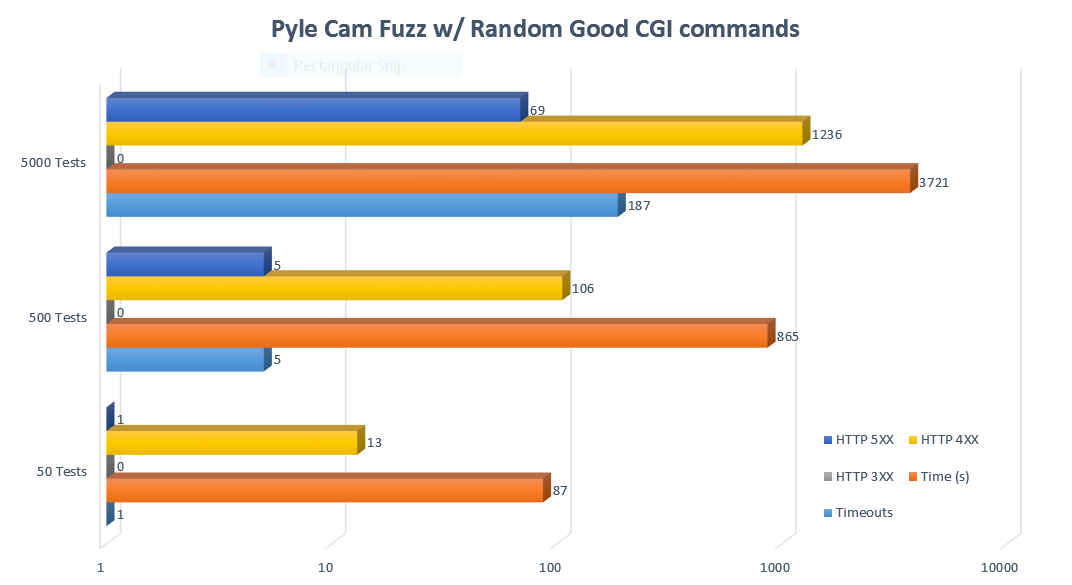
\includegraphics[width=0.9\linewidth]{Pyle_Good_CGI}
\caption{ 5550 fuzz tests on Pyle camera with valid commands}
\label{fig:Pyle_Good_CGI}
\end{figure*}

\begin{figure*}
\centering
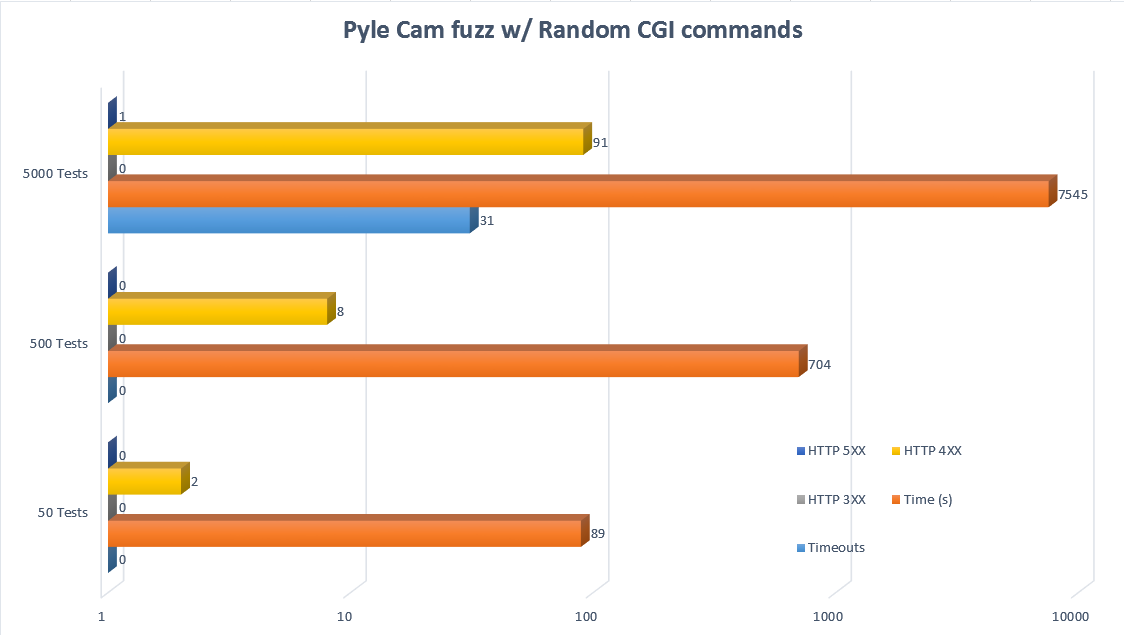
\includegraphics[width=0.9\linewidth]{Pyle_Rand_CGI}
\caption{5550 fuzz tests on Pyle camera with random commands}
\label{fig:Pyle_Rand_CGI}
\end{figure*}





{\footnotesize \bibliographystyle{acm}
\bibliography{biblio}}




\end{document}






